%% paper.tex — ACM eEnergy 2027 Fall submission draft
%% Double-blind review copy: sigconf + review + anonymous.
%% Source of truth for content is paper.md; keep the two in sync by hand
%% (paper.md is easier to edit/diff, this file is what actually compiles).
%% Fourth pivot (2026-09-09): coincidence-ceiling mechanism (\S4.6) supersedes the earlier
%% drf_power_tiebreak_full/lmetric_power headline; decision-noise-floor + metric-selection
%% methodology (\S5) added as a third pillar. See paper.md's status header for the full
%% rationale and ../findings/2026-08-31-eenergy-drf-lmetric-roundrobin-comparison.md Parts
%% 1-16 for every underlying number.
\documentclass[sigconf,review,anonymous]{acmart}
\usepackage{tikz}
\usetikzlibrary{arrows.meta,positioning}
\usepackage{enumitem}
\setlist[itemize]{itemsep=0.5pt,topsep=2pt,parsep=0pt,partopsep=0pt}
\usepackage{subcaption}
\setlength{\textfloatsep}{3pt plus 1pt minus 1pt}
\setlength{\floatsep}{2pt plus 1pt minus 1pt}
\setlength{\intextsep}{3pt plus 1pt minus 1pt}
\setlength{\abovecaptionskip}{2pt}
\setlength{\belowcaptionskip}{0pt}

\AtBeginDocument{%
  \providecommand\BibTeX{{Bib\TeX}}}

%% acmart defines `lemma`/`proof` via amsthm but not `claim`/`corollary`/`theorem`/
%% `proposition` -- needed for \S4.2's counterexample, \S4.3's corollary, and \S4.5's
%% egalitarian-vs-utilitarian results.
\newtheorem{claim}{Claim}
\newtheorem{corollary}{Corollary}
\newtheorem{theorem}{Theorem}
\newtheorem{proposition}{Proposition}

%% Rights-management placeholders — fill in from the rights-confirmation
%% email after acceptance. Not needed for the anonymous review submission.
\setcopyright{acmlicensed}
\copyrightyear{2027}
\acmYear{2027}
\acmDOI{XXXXXXX.XXXXXXX}
\acmConference[eEnergy '27]{ACM eEnergy 2027 Fall: 17th ACM International Conference on
  Future and Sustainable Energy Systems}{TBD 2027}{TBD}
\acmISBN{978-1-4503-XXXX-X/2027/TBD}

\begin{document}

\title{Fleet-Coincidence-Aware Power Routing: A Provably Safe Mechanism for Multi-GPU LLM Serving}

\author{Anonymous Author(s)}
\affiliation{%
  \institution{Anonymous Institution}
  \country{}
}

\begin{abstract}
We formalize power-aware request routing for multi-GPU LLM-serving fleets as a
multi-resource social welfare problem: each replica carries three independently-normalized
shares --- compute (prefix-cache-discounted prefill cost), load (in-flight request count),
and power (live NVML-measured ramp rate relative to a calibrated ceiling) --- and the router
seeks an egalitarian (max-min) welfare allocation across candidates at each routing decision,
extending Dominant Resource Fairness~\cite{ghodsi2011drf} to a third, reactive resource
dimension. We prove that routing via the fully-sorted lexicographic dominant-share rule
selects a Pareto-non-dominated candidate at every decision (verified against 200{,}000 random
instances with zero violations, in addition to a closed-form proof), and that this guarantee
extends unchanged to any shared, fleet-wide ceiling adjustment --- including a novel
\textbf{coincidence-ceiling} mechanism we introduce, which contracts every candidate's ramp
ceiling when multiple replicas are simultaneously elevated, directly targeting the
fleet-\emph{aggregate} coincident-ramp hazard that a purely per-replica signal cannot see. We
adopt the resulting rule, $\mathit{drf\_power\_tiebreak\_full\_coincidence\_ceiling}$, as our
proposed strategy, and show two natural alternatives --- a fixed-priority DRF tie-break, and
the same coincidence-ceiling mechanism applied to a power-extended LMETRIC score --- each
provably sacrifice the guarantee via distinct mechanisms. On real 8$\times$4090 hardware,
across 7 workload conditions including two real traces (BurstGPT, WildChat), our proposed
rule reduces peak power by 4.7\% relative to a power-blind baseline on the condition central
to this paper's motivation ($p{=}0.0017$, $n{=}6$), with TTFT and TBT directionally favorable
on the same condition but not independently significant at this trial count. Against the
strongest empirically-performing but \emph{not} Pareto-safe alternative, replicated to matched
$n{=}6$, the proposed rule is statistically indistinguishable across every metric measured in
this study --- peak power, TTFT, TBT, ramp-derivative statistics, energy-per-token, and
SLO-violation-rate: \textbf{the safety guarantee costs nothing on any axis we measure.} A
second, methodological contribution follows from this validation: we characterize a
${\sim}75$--85\% decision-level noise floor inherent to closed-loop real-hardware routing
evaluation (confirmed real via a state-blind control and real unpadded conversational traces,
not a workload artifact), identify which evaluation statistics survive it (metrics summing
over many independent events, e.g.\ energy-per-token, SLO-violation-rate) and which don't
(ramp derivatives, extreme-value statistics), and use this to determine which comparisons in
this line of work can currently be trusted.
\end{abstract}

\begin{CCSXML}
<ccs2012>
   <concept>
       <concept_id>10010147.10010919.10010920.10010921</concept_id>
       <concept_desc>Computer systems organization~Cloud computing</concept_desc>
       <concept_significance>500</concept_significance>
   </concept>
   <concept>
       <concept_id>10010147.10010919.10010172</concept_id>
       <concept_desc>Computer systems organization~Dependable and fault-tolerant systems and networks</concept_desc>
       <concept_significance>300</concept_significance>
   </concept>
   <concept>
       <concept_id>10003752.10003809.10010031</concept_id>
       <concept_desc>Theory of computation~Scheduling algorithms</concept_desc>
       <concept_significance>300</concept_significance>
   </concept>
</ccs2012>
\end{CCSXML}

\ccsdesc[500]{Computer systems organization~Cloud computing}
\ccsdesc[300]{Computer systems organization~Dependable and fault-tolerant systems and networks}
\ccsdesc[300]{Theory of computation~Scheduling algorithms}

\keywords{LLM serving, request routing, power management, dominant resource fairness,
  Pareto optimality, data center energy, evaluation methodology}

\maketitle

\section{Introduction}

\textbf{Motivation.} Multi-GPU LLM-serving fleets draw power in bursts as requests arrive and
complete, and the resulting ramp volatility --- not just mean draw --- is a concern for
facility power delivery and, at larger scale, for grid-facing demand response. This paper
addresses the fleet-internal version of that hazard: coincident power-ramp spikes across
replicas within a single serving fleet, a risk that grows with fleet size and is invisible to
any policy that reasons about replicas independently. The request router, the component
deciding which replica serves each incoming request, is a free lever against this hazard: no
hardware change, no compute cost, just a policy. This paper asks a precise question about that
lever: \emph{can we route in a way that
is provably fair/efficient across resources and defends against \textbf{fleet-wide coincident}
power-ramp hazards specifically, and --- since natural power-aware deviations from a provably
safe rule turn out to sacrifice the guarantee --- do we actually have to give up that
guarantee to get a power-aware win in practice, or does the safe rule already deliver one for
free?}

\begin{figure}[t]
  \centering
  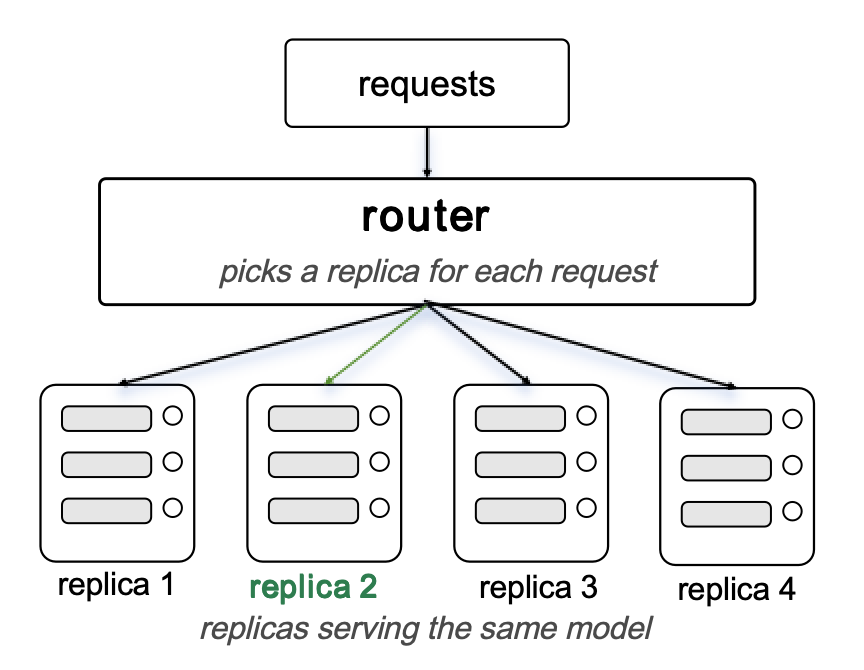
\includegraphics[width=0.5\linewidth]{figs/LLM_routing_illustration.png}
  \caption{The setting this paper targets: a router dispatches each incoming request to one
    of several replicas serving the same model.}
  \label{fig:setting}
\end{figure}

\textbf{Contributions.}
\begin{enumerate}
  \item A formalization of power-aware LLM-serving routing as a 3-resource
    (compute/load/power) egalitarian social welfare problem extending DRF~\cite{ghodsi2011drf}
    to a reactive, time-varying power dimension (\S\ref{sec:formulation}), and a proof the
    natural sorted-lexicographic solution is Pareto-non-dominated at every decision
    (\S\ref{sec:lemma1}).
  \item \textbf{The coincidence-ceiling mechanism} (\S\ref{sec:coincidence-ceiling}): a
    pluggable, fleet-aware extension contracting every candidate's ramp ceiling by a single
    shared scalar when multiple replicas are simultaneously elevated --- targeting the
    fleet-\emph{aggregate} coincident-ramp hazard no purely per-replica rule can see. Requires
    no new safety proof (a direct instantiation of \S\ref{sec:ceiling-invariance}) and
    generalizes across rule families, inheriting each parent's own safety status. We adopt
    $\mathit{drf\_power\_tiebreak\_full\_coincidence\_ceiling}$
    ($\mathit{coincidence\_ceiling}$) as this paper's proposed strategy.
  \item Two proofs, via explicit counterexample, that natural alternatives sacrifice the
    guarantee via distinct mechanisms: a fixed-priority power tie-break, repaired by
    appending the dropped resource rather than truncating it, and a power-extended LMETRIC
    score whose multiplicative structure collapses to an uninformative tie on any full
    prefix-cache hit (12.8\% of realistic instances, \S\ref{sec:counterexample}).
  \item Real-hardware validation on an 8$\times$4090 fleet across 7 workload conditions
    (two real traces): a significant peak-power reduction relative to a power-blind baseline
    on the condition motivating this paper ($p{=}0.0017$, $n{=}6$), with TTFT and TBT
    directionally favorable but not independently significant at this trial count
    (\S\ref{sec:eval-dominance}); and, against the strongest empirically-performing but
    \emph{not} Pareto-safe alternative, replicated to matched $n{=}6$, no statistically
    distinguishable difference on any metric measured: peak power, TTFT, TBT,
    ramp-derivative statistics, energy-per-token, or SLO-violation-rate
    (\S\ref{sec:eval-dominance}--\S\ref{sec:eval-matched}). The guarantee is free on every
    axis tested.
  \item \textbf{A decision-level noise-floor characterization and evaluation methodology}
    (\S\ref{sec:methodology}), useful beyond this paper: real-hardware closed-loop routing
    evaluation carries a ${\sim}75$--85\% per-decision mismatch between two runs of the
    \emph{identical} policy, driven by non-reproducible hardware timing rather than workload
    construction (\S\ref{sec:noisefloor}); we identify which aggregate statistics survive this
    noise at feasible trial counts and which don't (\S\ref{sec:metricselection}), determining
    which of this paper's own claims can be asserted with confidence
    (\S\ref{sec:trialcount}, \S\ref{sec:eval}).
\end{enumerate}

\textbf{Roadmap.} Three normalized shares (compute, load, power, \S\ref{sec:formulation}) feed
a sorted rule, proven Pareto-safe (Lemma~\ref{lem:sorted-nondominated}, \S\ref{sec:lemma1}).
Two natural power-biased variants of it sacrifice that guarantee: a fixed-priority tie-break
(Claim~\ref{claim:named-rule}, repaired into $\mathit{drf\_power\_tiebreak\_full}$) and a
power-extended LMETRIC score (Claim~\ref{claim:lmetric-power}, 12.8\% of realistic instances,
\S\ref{sec:counterexample}); $\mathit{weighted\_sum}$ is a structurally different Pareto-safe
alternative that is not threshold-safe for any weights
(Theorem~\ref{thm:impossibility}, \S\ref{sec:leximin}). The coincidence-ceiling mechanism
(\S\ref{sec:coincidence-ceiling}) applies to all three, inheriting rather than granting safety
status, and yields this paper's proposed rule,
$\mathit{drf\_power\_tiebreak\_full\_coincidence\_ceiling}$. On real 8$\times$4090 hardware
(\S\ref{sec:eval}) it delivers a significant peak-power reduction vs.\ $\mathit{lmetric}$
(power-blind) on the short/original condition ($p{=}0.0017$, Table~\ref{tab:headline}) and is
statistically indistinguishable from the strongest empirically-performing but unsafe
alternative on every metric measured at matched $n{=}6$
(Table~\ref{tab:energyslo}, \S\ref{sec:eval-matched}).
Table~\ref{tab:rules} gives the full safety status of every rule discussed, including
$\mathit{drf\_fixed}$ and $\mathit{round\_robin}$.

\vspace{-3pt}
\section{Problem Formulation}
\label{sec:formulation}

Consider $N$ replicas serving requests behind a router. For a candidate replica $c$ and an
incoming request, define three shares, each normalized to roughly $[0,\infty)$ with $1.0$
representing ``at capacity'':

\begin{itemize}
  \item $\mathit{Share_{compute}}(c) = \mathit{P\text{-}token}(c) / \mathit{token\_budget}(c)$
    --- $\mathit{P\text{-}token}$ is the prefix-cache-discounted count of \emph{new} prefill
    tokens this request would cost replica $c$ (computed from a per-replica cache-state
    mirror), so this share already reflects cache locality, not raw prompt length.
  \item $\mathit{Share_{load}}(c) = \mathit{in\_flight\_after}(c) / \mathit{max\_num\_seqs}(c)$
    --- in-flight request count after dispatch, normalized to the replica's configured
    concurrency limit.
  \item $\mathit{Share_{power}}(c) = \max(\mathit{ramp\_rate}(c), 0) / \mathit{ramp\_ceiling}(c)$
    --- the replica's own currently NVML-measured power-ramp rate, normalized to a calibrated
    per-GPU ceiling. Clamped to non-negative because a routing decision can only ever push
    the \emph{receiving} replica's power up, never down --- a falling ramp is not a
    decision-relevant hazard for routing purposes. ($\mathit{ramp\_ceiling}$ itself is
    physically grounded in the GPU's own DVFS transition dynamics --- \S\ref{sec:relatedwork}
    relates the two explicitly.)
\end{itemize}

\textbf{Departure from DRF's original model.} Ghodsi et al.'s DRF~\cite{ghodsi2011drf}
assumes a fixed, known demand vector per user, allocated from a fixed resource pool.
$\mathit{Share_{power}}$ is neither: it is a live, exogenously-evolving measurement of the
replica's \emph{own current state}, not a declared demand of the request being routed, and it
changes between routing decisions independent of routing choices. We do not assume the
original static-demand Pareto-efficiency proof transfers to this setting --- \S\ref{sec:lemma1}
proves the property we actually need (per-decision, not per-trajectory) directly for this
model.

\textbf{Why $\mathit{Share_{power}}$ is a state read, not a projection.}
$\mathit{Share_{compute}}$ and $\mathit{Share_{load}}$ are one-step projections attributable
to the specific request being routed: $P\text{-}token$ is \emph{this request's} incremental
prefill cost, and $\mathit{in\_flight\_after}$ is the queue depth \emph{after this request is
hypothetically added}. $\mathit{Share_{power}}$ cannot be given the same treatment: a GPU's
instantaneous power draw is an emergent property of whatever batch is currently executing,
not a quantity linearly attributable to any single request, so there is no well-defined
``ramp rate after this request'' the way there is a well-defined queue depth after it. What we
read instead is the replica's \emph{current} state --- exactly the object a rate limiter reads
in classical feedback control~\cite{astrom2008feedback}, and exactly the kind of signal
classical state-dependent load balancing (power-of-two-choices,
join-shortest-queue)~\cite{mitzenmacher2001power, azar1994balanced} routes on: an observed
state, not a computed causal attribution. None of \S\ref{sec:lemma1}--\S\ref{sec:coincidence-ceiling}'s
guarantees depend on this distinction --- every proof treats $s(c)$ as an arbitrary comparable
real vector available at decision time, regardless of whether a coordinate is a
request-specific projection or a current-state read. The distinction does, however, determine
how the two kinds of metric must be evaluated: TTFT and TBT are per-decision outcomes,
decomposable into a population of independent per-request measurements the way
$\mathit{Share_{compute}}$ and $\mathit{Share_{load}}$ are decomposable into per-request costs;
power and ramp are properties of the continuous trajectory the routing policy induces over
time, evaluable only in aggregate, the same way a feedback controller is evaluated by its
closed-loop trajectory (peak deviation, settling time) rather than by attributing trajectory
segments to individual control actions. \S\ref{sec:methodology}--\S\ref{sec:eval} evaluate them
accordingly, and \S\ref{sec:noisefloor}--\S\ref{sec:metricselection} show this ``aggregate-only''
evaluability is exactly why ramp statistics are harder to trust at low trial counts than
per-request statistics are.

\textbf{Welfare objective.} At each routing decision, define the dominant share
$D(c) = \max(\mathit{Share_{compute}}(c), \mathit{Share_{load}}(c), \mathit{Share_{power}}(c))$.
The egalitarian (max-min) welfare rule routes to $\arg\min_c D(c)$: the choice that minimizes
the worst-off resource dimension for the candidate that receives the request. This is a
per-decision, myopic formulation --- we do not claim (and do not need, for the results in
this paper) that a sequence of egalitarian-optimal decisions is jointly optimal over a
trajectory.

\begin{figure}[t]
  \centering
  \begin{subfigure}[b]{\linewidth}
    \centering
    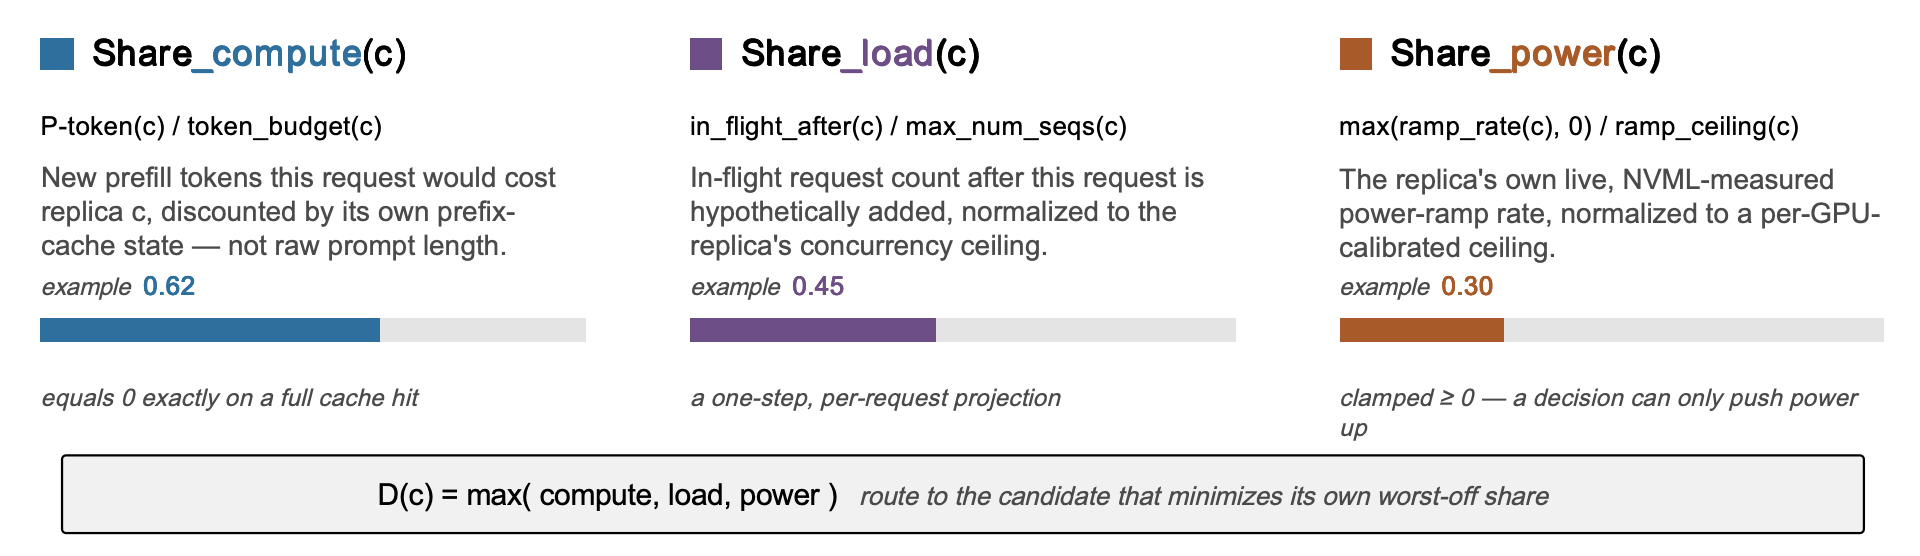
\includegraphics[width=\linewidth]{figs/overview_2.png}
    \caption{The three normalized shares and the dominant share $D(c)$, with representative
      example values for one candidate replica.}
    \label{fig:shares}
  \end{subfigure}
  \par\vspace{1pt}
  \begin{subfigure}[b]{\linewidth}
    \centering
    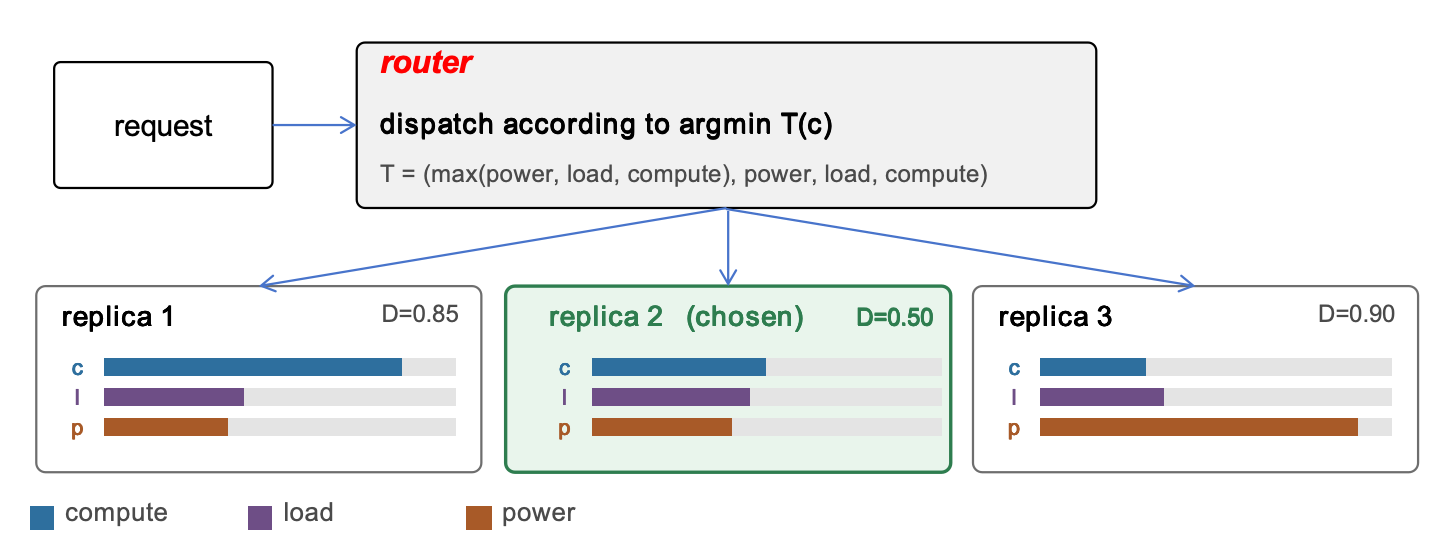
\includegraphics[width=0.95\linewidth]{figs/overview_1.png}
    \caption{Routing a single request under the full tie-break vector $T(c)$ formalized in
      \S\ref{sec:counterexample}: the router evaluates each replica's tuple and dispatches to
      the $\arg\min$ (replica 2 here, despite not having the lowest individual share on every
      coordinate).}
    \label{fig:routing-example}
  \end{subfigure}
  \caption{From shares to a routing decision.}
  \label{fig:shares-and-routing}
\end{figure}

\vspace{-3pt}
\section{Theory}

\subsection{The sorted-lexicographic rule is Pareto-non-dominated}
\label{sec:lemma1}

$\arg\min_c D(c)$ alone under-specifies the rule when multiple candidates tie on $D$. Define
the \textbf{sorted rule}: route to $\arg\min_c \sigma(s(c))$, where
$s(c) = (\mathit{Share_{compute}}(c), \mathit{Share_{load}}(c), \mathit{Share_{power}}(c))$,
$\sigma$ sorts a vector into descending order, and ties are broken by standard lexicographic
comparison of the sorted vectors.

\begin{lemma}
\label{lem:sorted-nondominated}
The candidate selected by the sorted rule is Pareto-non-dominated among the candidate set: no
other candidate $c'$ satisfies $\mathit{Share}_i(c') \le \mathit{Share}_i(c^*)$ for all three
resources $i$ with strict inequality for at least one.
\end{lemma}

\begin{proof}
For $v \in \mathbb{R}^3$, write $v_{(1)} \ge v_{(2)} \ge v_{(3)}$ for its order statistics, so
$\sigma(v) = (v_{(1)}, v_{(2)}, v_{(3)})$. Suppose toward contradiction that $c'$
Pareto-dominates $c^* = \arg\min_c \sigma(s(c))$: $s(c') \le s(c^*)$ coordinatewise, with
strict inequality at some coordinate $i_0$.

\emph{(i) $\sigma(s(c')) \le \sigma(s(c^*))$ coordinatewise.} For any threshold $t$ and any
$i$, $s(c')_i \ge t \Rightarrow s(c^*)_i \ge s(c')_i \ge t$, so
$\#\{i : s(c')_i \ge t\} \le \#\{i : s(c^*)_i \ge t\}$. The $k$-th order statistic is the
least $t$ with $\#\{i : v_i \ge t\} \ge k$; a pointwise-smaller counting function cannot raise
this threshold, so $s(c')_{(k)} \le s(c^*)_{(k)}$ for every $k$.

\emph{(ii) The inequality is strict as vectors.} Sorting permutes coordinates, so
$\sum_k s(c')_{(k)} = \sum_i s(c')_i < \sum_i s(c^*)_i = \sum_k s(c^*)_{(k)}$, the middle
inequality from domination at $i_0$. Hence $\sigma(s(c')) \ne \sigma(s(c^*))$.

\emph{(iii) Lexicographic order.} Two coordinatewise-$\le$ vectors that differ somewhere are
ordered lexicographically at their first differing coordinate, in the direction of (i)'s
inequality there: $\sigma(s(c')) <_{\mathrm{lex}} \sigma(s(c^*))$.

\emph{(iv)} The sorted rule then selects $c'$ over $c^*$, contradicting $c^*$'s selection.
\end{proof}

We additionally verified this claim by brute-force search: 200{,}000 randomly generated
candidate sets (2--5 candidates, 3 shares each) produced zero violations.

\subsection{Two natural variants sacrifice the guarantee, via two distinct mechanisms}
\label{sec:counterexample}

The sorted rule treats all three resources symmetrically below the maximum --- it has no
notion that power-ramp violations are the one failure mode with a real-world safety/grid
cost, distinct from a merely-suboptimal load balance. This motivates two independent, natural
attempts to bias the rule toward power specifically. We show both provably sacrifice
Lemma~\ref{lem:sorted-nondominated}'s guarantee, via mechanisms different enough that
neither's fix addresses the other --- itself evidence that the guarantee is a real structural
constraint worth checking explicitly for any new score design, not a formality.

\textbf{Fixed-priority power tie-break.} A natural fix to the sorted rule: after comparing
the dominant share, always compare $\mathit{Share_{power}}$ next, \emph{by name}, ahead of
$\mathit{Share_{load}}$, regardless of which is numerically larger. Define the \textbf{named
rule}: route to $\arg\min_c (D(c), \mathit{Share_{power}}(c), \mathit{Share_{load}}(c))$
under standard lexicographic order.

\begin{claim}
\label{claim:named-rule}
The named rule can select a Pareto-dominated candidate.
\end{claim}

\textbf{Construction.} Let candidates $A$ and $B$ be given, in
$(\mathit{Share_{compute}}, \mathit{Share_{load}}, \mathit{Share_{power}})$ form, by
\[
  A = (0.3,\ 0.9,\ 0.9), \qquad B = (0.5,\ 0.9,\ 0.9).
\]
$A$ Pareto-dominates $B$ (equal load and power, strictly lower compute). Both have $D(A) = D(B) = 0.9$ and
identical $\mathit{Share_{power}}$ and $\mathit{Share_{load}}$, so the named rule's 3-tuple
$(D, \mathit{Share_{power}}, \mathit{Share_{load}})$ is \emph{identical} for $A$ and $B$ ---
the rule cannot see the compute difference at all, since compute only enters through $D$, and
$D$ is tied. $\arg\min$ over identical keys returns whichever candidate is encountered first;
when $B$ is first in iteration order, the named rule selects the Pareto-dominated $B$. This
was verified directly in code, not only argued: a brute-force check across 200{,}000 random
instances reproduces the failure mode.

\textbf{Why this happens.} The named rule buys a deliberate, domain-motivated priority ---
never let a load difference override a power difference --- at the cost of the compute
dimension becoming invisible whenever the dominant share is tied via load or power rather
than compute: $\mathit{Share_{compute}}$ never appears anywhere in the 3-tuple
$(D, \mathit{Share_{power}}, \mathit{Share_{load}})$, so once $D$, $\mathit{Share_{power}}$,
and $\mathit{Share_{load}}$ all tie, the rule has no remaining information to break the tie
correctly.

\begin{figure}[t]
  \centering
  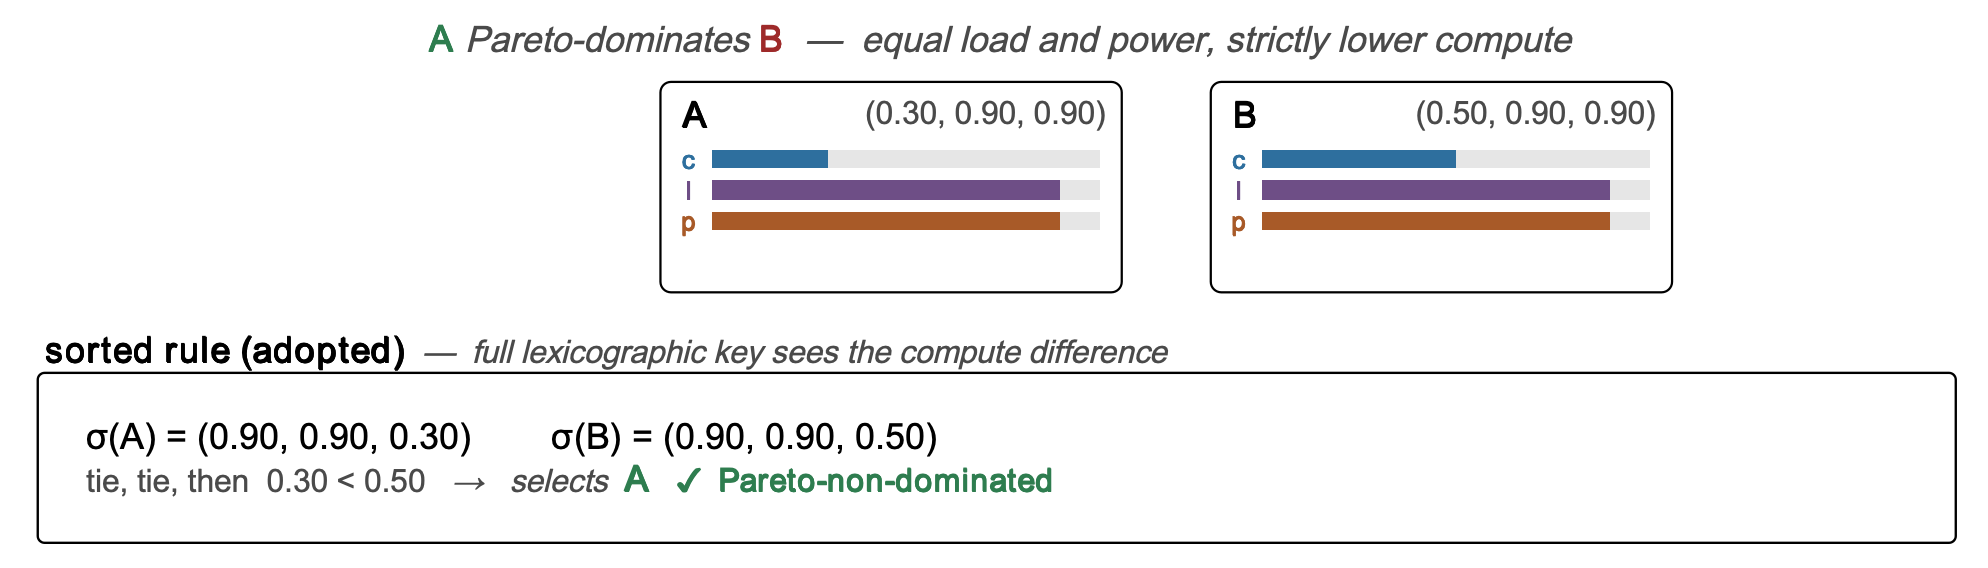
\includegraphics[width=\linewidth]{figs/pareto_dominance.png}
  \caption{The same $A$/$B$ pair the named rule fails on: the full lexicographic key used by
    the sorted rule this paper adopts sees the compute difference the named rule's truncated
    tuple cannot, and correctly selects the Pareto-non-dominated candidate $A$.}
  \label{fig:pareto-dominance}
\end{figure}

\textbf{The repair, and this paper's base rule.} The fix is to stop truncating the tuple:
append $\mathit{Share_{compute}}$ as an explicit fourth coordinate rather than dropping it.
Define $T(c) = (D(c), \mathit{Share_{power}}(c), \mathit{Share_{load}}(c),
\mathit{Share_{compute}}(c))$ and route to $\arg\min_c T(c)$. This keeps the exact same
primary criterion and the same deliberate power-before-load priority the named rule was
built for --- it changes nothing about \emph{when} power is allowed to override load --- it
only ensures no coordinate is ever silently dropped. We call this rule
\texttt{drf\_power\_tiebreak\_full}; \S\ref{sec:coincidence-ceiling} extends it with the
coincidence-ceiling mechanism to produce this paper's actual proposed strategy.



\begin{corollary}
\label{cor:tiebreak-full-safe}
$\arg\min_c T(c)$ is Pareto-non-dominated at every decision.
\end{corollary}

\begin{proof}
Write $s = (\mathit{Share_{compute}}, \mathit{Share_{load}}, \mathit{Share_{power}})$ and
suppose $c'$ Pareto-dominates $c^* = \arg\min_c T(c)$: $s(c') \le s(c^*)$ coordinatewise,
strict somewhere. $D = \max(s)$ is monotone under coordinatewise $\le$, so
$D(c') \le D(c^*)$. Three exhaustive cases:
\begin{itemize}
  \item \textbf{$D(c') < D(c^*)$.} $T(c') <_{\mathrm{lex}} T(c^*)$ at coordinate 1.
  \item \textbf{$D(c') = D(c^*)$, and $\mathit{Share_{power}}(c') \le \mathit{Share_{power}}(c^*)$
    strict.} $T(c') <_{\mathrm{lex}} T(c^*)$ at coordinate 2. (Symmetrically for
    $\mathit{Share_{load}}$ at coordinate 3, if $D$ and $\mathit{Share_{power}}$ tie but
    $\mathit{Share_{load}}$ does not.)
  \item \textbf{$D$, $\mathit{Share_{power}}$, $\mathit{Share_{load}}$ all tied between $c'$
    and $c^*$.} Domination requires a strict inequality in $s(c') \le s(c^*)$; the first
    three coordinates being tied forces it onto $\mathit{Share_{compute}}$:
    $\mathit{Share_{compute}}(c') < \mathit{Share_{compute}}(c^*)$, so
    $T(c') <_{\mathrm{lex}} T(c^*)$ at coordinate 4.
\end{itemize}
Every case gives $T(c') <_{\mathrm{lex}} T(c^*)$, contradicting $c^*$'s selection as
$\arg\min_c T(c)$.
\end{proof}

This closed-form proof is in fact simpler than Lemma~\ref{lem:sorted-nondominated}'s, since a
fixed coordinate order needs no rearrangement argument. Direct verification in code confirms
it resolves Claim~\ref{claim:named-rule}'s exact counterexample under both iteration orders,
while the plain named rule still fails it (200{,}000 trials, 0 violations).

\textbf{Power-extended LMETRIC.} A different, non-DRF way to add a power signal: extend
LMETRIC's own multiplicative score, $\mathit{new\_tokens} \times \mathit{in\_flight\_after}$,
with a continuous power penalty, $(1 + \mathit{Share_{power}})$. Restated in this paper's
normalized shares (holding $\mathit{token\_budget}$ and $\mathit{max\_num\_seqs}$ fixed
across candidates, so raw counts equal shares), this is $\mathit{lmetric\_power}(c) =
\mathit{Share_{compute}}(c) \cdot \mathit{Share_{load}}(c) \cdot (1 +
\mathit{Share_{power}}(c))$, routing to the minimum. This is the routing analogue of Lyapunov
drift-plus-penalty scheduling~\cite{neely2010stochastic} --- a soft, ever-present penalty
rather than a hard constraint --- and the path of least engineering resistance for anyone
already running LMETRIC: one multiplicative factor on an existing score, no new normalization
or tie-break design. We check this specific variant precisely because it is the one an
engineer would reach for first, not a foil constructed to fail.

\begin{claim}
\label{claim:lmetric-power}
$\mathit{lmetric\_power}$ can select a Pareto-dominated candidate, via a different mechanism
than Claim~\ref{claim:named-rule}: any candidate with $\mathit{Share_{compute}} = 0$ (a full
prefix-cache hit --- no new tokens to prefill) scores exactly $0$, \emph{regardless of its
load or power share}. Two such candidates are indistinguishable to the score no matter how
different their load and power are.
\end{claim}

\textbf{Construction.} Let $A = (0.0, 0.1, 0.1)$ and $B = (0.0, 0.9, 0.9)$ --- both cache
hits; $A$ strictly Pareto-dominates $B$ on both load and power.
$\mathit{lmetric\_power}(A) = \mathit{lmetric\_power}(B) = 0$. With $B$ first in iteration
order, $\arg\min$ selects the Pareto-dominated $B$, verified directly in code.

This mechanism is qualitatively different from Claim~\ref{claim:named-rule}'s: it requires an
\emph{exact} tie in $\mathit{Share_{compute}}$, but $\mathit{Share_{compute}} = 0$ is not
measure-zero in real traffic --- it is a common, discrete event (a full prefix-cache hit), and
this paper's own Light/Cachehit condition (\S\ref{sec:eval}) is specifically constructed to
be dominated by it. Sampling at a realistic cache-hit rate (40\%, matching Light/Cachehit's
rough hit rate) over 200{,}000 random instances (2--5 candidates) finds 25{,}618 violations
--- \textbf{12.8\% of instances}, not a rare corner case.

\textbf{A structurally different safe alternative.} $\mathit{weighted\_sum}(c) =
0.33 \cdot \mathit{Share_{compute}}(c) + 0.33 \cdot \mathit{Share_{load}}(c) + 0.33 \cdot
\mathit{Share_{power}}(c)$, route to the minimum, is a classical result
\cite{geoffrion1968proper}: any positive-weighted linear combination of the shares preserves
Pareto non-domination. This was verified for the specific weights used here (200{,}000
trials, 0 violations) so that \S\ref{sec:eval} can include it as an \emph{external validity
check}: a safe rule built on an entirely different mechanism, included specifically to show
that any empirical result about giving up the Pareto guarantee is not an artifact of this
paper's own DRF-based construction.

\textbf{A family of Pareto-safe repairs of $\mathit{lmetric\_power}$ itself was also
considered and not adopted:} $\mathit{lmetric\_power\_pareto}$, replacing the
multiplicative form with $(\mathit{shift} + \mathit{Share_{compute}}) \cdot
(\mathit{shift} + \mathit{Share_{load}}) \cdot (\mathit{shift} + \mathit{Share_{power}})$,
which removes Claim~\ref{claim:lmetric-power}'s zero-collapse by construction (every factor
strictly positive whenever $\mathit{shift} > 0$) and is Pareto-safe by the same
monotone-product argument that makes $\mathit{weighted\_sum}$ safe (verified, 200{,}000
trials, 0 violations at $\mathit{shift}{=}1$ and several tested $\mathit{shift}{=}\varepsilon$
values). This family is \textbf{not threshold-safe for the same reason $\mathit{weighted\_sum}$
isn't}: Theorem~\ref{thm:impossibility} (\S\ref{sec:leximin}) rules out threshold-safety for
\emph{any} fixed-weight or fixed-shift multiplicative construction, so no choice of shift can
ever match Theorem~\ref{thm:threshold-safety}'s guarantee. Its apparent empirical edge over
the proposed rule at low trial counts did not survive the noise-band audit in
\S\ref{sec:trialcount}; it is not adopted as a headline alternative.

\textbf{What \S\ref{sec:eval} tests, and each arm's role there.} Table~\ref{tab:rules}
summarizes every rule this paper discusses and its safety status in one place; none are
interchangeable in role even where two share a safety guarantee.

\begin{table*}[t]
  \caption{Routing rules discussed in this paper, at a glance. ``Threshold-safe'' extends
    Theorem~\ref{thm:threshold-safety}'s guarantee to any rule that sorts on $D$ first.
    Coincidence-ceiling variants (\S\ref{sec:coincidence-ceiling}) inherit their parent
    rule's status unchanged --- the mechanism generalizes safety status, it does not grant
    it.}
  \label{tab:rules}
  \footnotesize
  \setlength{\tabcolsep}{5pt}
  \begin{tabular}{@{}llccl@{}}
    \toprule
    Rule & Family & Pareto-safe & Thresh.-safe & Role \\
    \midrule
    \texttt{drf\_fixed} & sorted (leximin) & \checkmark~(Lem.~\ref{lem:sorted-nondominated}) & \checkmark & unmodified baseline \\
    \texttt{drf\_power\_tiebreak\_full} & sorted (leximin) & \checkmark~(Cor.~\ref{cor:tiebreak-full-safe}) & \checkmark & base repair, not proposed directly \\
    \texttt{..\_coincidence\_ceiling} & sorted + shared ceiling & \checkmark~(\S\ref{sec:coincidence-ceiling}) & \checkmark & \textbf{proposed} (\texttt{coincidence\_ceiling}) \\
    \texttt{drf\_power\_tiebreak} (named) & sorted, truncated tie-break & $\times$~(Claim~\ref{claim:named-rule}) & \checkmark & motivates the repair \\
    \texttt{weighted\_sum} & utilitarian (linear) & \checkmark~\cite{geoffrion1968proper} & $\times$~(Thm.~\ref{thm:impossibility}) & external validity check \\
    \texttt{weighted\_sum\_coincidence\_ceiling} & utilitarian + shared ceiling & \checkmark~(\S\ref{sec:coincidence-ceiling}) & $\times$~(Thm.~\ref{thm:impossibility}) & ext.\ check, coincidence-aware \\
    \texttt{lmetric\_power} & multiplicative & $\times$~(Claim~\ref{claim:lmetric-power}) & $\times$ & unsafe baseline \\
    \texttt{lmetric\_power\_coincidence\_ceiling} & multiplicative + shared ceiling & $\times$~(unaffected) & $\times$ & \textbf{strongest unsafe alt.} --- \S\ref{sec:eval}'s comparator \\
    \texttt{lmetric\_power\_pareto} ($+\varepsilon$) & shifted-product & \checkmark & $\times$~(Thm.~\ref{thm:impossibility}) & explored, not adopted \\
    \texttt{lmetric} (power-blind) & multiplicative, no power & n/a & n/a & power-blind baseline \\
    \texttt{round\_robin} & blind (no signal) & n/a & n/a & state-blind floor \\
    \bottomrule
  \end{tabular}
\end{table*}

Against this backdrop, the empirical question \S\ref{sec:eval} asks is whether giving up the
Pareto guarantee --- via $\mathit{lmetric\_power\_coincidence\_ceiling}$, the \emph{strongest
empirically-performing} alternative found anywhere in this project's testing (it out-dominates
every other tested arm more than 3-to-1 in raw pairwise tally) --- buys anything a provably
safe rule does not already deliver. This strongest-known unsafe alternative, not a weaker
foil, is deliberately used as the comparator, so that any advantage in its favor would be the
most convincing evidence available; \S\ref{sec:eval} finds no such advantage on the metrics
that survive \S\ref{sec:methodology}'s noise-floor scrutiny.

\subsection{A live-calibrated ceiling preserves the guarantee, and requires it to be shared}
\label{sec:ceiling-invariance}

Both rules above assume $\mathit{Share_{power}}(c) = \max(\mathit{ramp\_rate}(c),0) / \kappa$
for a fixed constant ceiling $\kappa$ (per-GPU calibrated, \S\ref{sec:methodology}). A natural
objection: does either guarantee survive replacing $\kappa$ with a value recalibrated live
from the fleet's own recent state --- as an \emph{adaptive-ceiling} variant of either rule
(and, as \S\ref{sec:coincidence-ceiling} shows, the coincidence-ceiling mechanism itself)
would need?

\begin{corollary}
\label{cor:ceiling-invariance}
Lemma~\ref{lem:sorted-nondominated} holds unchanged for any $\kappa(t) > 0$ that is a single
scalar shared identically by every candidate at decision time $t$, regardless of how $\kappa(t)$
is computed --- static, adaptively recalibrated from fleet history, or otherwise.
\end{corollary}

\begin{proof}
The proof of Lemma~\ref{lem:sorted-nondominated} treats $s(c)$'s three coordinates as arbitrary
reals; it never uses the fact that $\mathit{Share_{power}}$'s denominator is constant
\emph{across} decisions, only that it is the same value for every candidate \emph{within} one
decision, so the coordinate remains a well-defined, comparable per-candidate quantity for that
decision's $\arg\min$. Substituting $\kappa(t)$ for a fixed constant changes nothing the proof
relies on.
\end{proof}

This was verified directly, not just by inspection of the proof: re-running
\S\ref{sec:lemma1}'s brute-force search with the ceiling itself independently randomized per
trial (not just the raw shares) still produces zero violations across 200{,}000 trials.
\textbf{\S\ref{sec:coincidence-ceiling}'s coincidence-ceiling mechanism is a direct
instantiation of this corollary}, not a separate result requiring its own proof.

\textbf{Sharing is load-bearing.} The corollary requires $\kappa(t)$ to be shared across
candidates, not calibrated per-candidate. Under a per-candidate $\kappa_c$, share-space
non-domination can dissociate from physical reality: two candidates with identical
compute/load but $(\mathit{raw\_ramp}, \kappa) = (0.9,\ 10)$ and $(0.1,\ 0.1)$ realize
$\mathit{Share_{power}} = 0.09$ and $1.0$ respectively --- the sorted rule (correctly, per
Lemma~\ref{lem:sorted-nondominated}) selects the first candidate as share-space
non-dominated, even though it draws the physically \emph{larger} raw ramp. This is why the
implementation instantiates one ceiling/coincidence-factor calibrator per router, not one per
replica.

\subsection{Round-filtered calibration is insensitive to concentration, not merely less sensitive}
\label{sec:ceiling-boundedness}

A live ceiling introduces its own hazard: a naive scheme that folds every observed ramp reading
into a rolling percentile is self-defeating under sustained multi-replica pressure ---
concentration (2+ replicas simultaneously elevated) is exactly the condition that fills the
window with elevated values, so the ceiling inflates \emph{most} during the episodes it is
supposed to guard against. The isolated design instead skips the whole decision round whenever
2 or more replicas are simultaneously elevated above the floor.

\begin{lemma}
\label{lem:insensitivity}
Let two fleet ramp-reading histories agree on every decision round with fewer than 2
simultaneously-elevated replicas, and differ arbitrarily on rounds with 2 or more. The
round-filtered calibration produces identical ceiling trajectories on both histories at every
timestep.
\end{lemma}

\begin{proof}
The round-filtered calibrator returns without modifying its window whenever a round's elevated
count is $\ge 2$; the ceiling is a deterministic function (a fixed percentile) of the window's
contents alone. Since the two histories only ever differ on rounds that are skipped entirely,
the window's contents --- and hence the ceiling --- are identical at every step.
\end{proof}

This was verified over 2{,}000 randomized paired-history trials (concentration-round
magnitudes scaled by a random factor up to $1000\times$ between the paired sequences): zero
violations. Feeding the identical paired histories through the naive (unfiltered,
per-observation) calibration instead diverges in every one of the 2{,}000 trials.

\subsection{Selecting among multiple Pareto-optimal points: egalitarian vs.\ utilitarian}
\label{sec:leximin}

Lemma~\ref{lem:sorted-nondominated} and Corollary~\ref{cor:tiebreak-full-safe} guarantee
membership on the Pareto frontier but say nothing about \emph{which} frontier point to prefer
when several candidates are mutually non-dominated --- a real question, since
$\mathit{weighted\_sum}$ (\S\ref{sec:counterexample}) is provably on the frontier too, by an
entirely different mechanism.

\textbf{The sorted rule is leximin.} The order $u \preceq v \iff \sigma(u) \le_{\mathrm{lex}}
\sigma(v)$ on share vectors is the classical \emph{leximin} (lexicographic egalitarian)
order~\cite{sen1970collective}: compare the worst coordinate first, then the second-worst, and
so on. Lemma~\ref{lem:sorted-nondominated}'s proof already establishes more than the lemma
states: domination strictly worsens a candidate's leximin rank, so the sorted rule computes
the leximin-minimal point. $\mathit{weighted\_sum}$ implements the classical
\emph{utilitarian} rule instead, $\arg\min_c \sum_i \mathit{Share}_i(c)$, also on the
frontier~\cite{geoffrion1968proper}, for a different, formally separable reason.

\textbf{Egalitarian rules reward equalization; utilitarian rules are blind to it.} For
$s(c) = (a,b,d)$ with $a$ the strict max, transferring $\varepsilon \in (0, (a-b)/2]$ from the
max coordinate to a smaller one without crossing strictly lowers the sorted rule's key but
leaves $\mathit{weighted\_sum}$ exactly unchanged --- the Pigou--Dalton transfer principle
(verified over 16{,}781 random transfers, 0 failures).

\begin{lemma}[Divergence]
\label{lem:divergence}
Let $X, Y$ be candidates with $D(X) < D(Y)$ and $\sum_i \mathit{Share}_i(X) > \sum_i
\mathit{Share}_i(Y)$. Then $X$ and $Y$ are Pareto-incomparable, the sorted rule selects $X$,
and $\mathit{weighted\_sum}$ selects $Y$. Whenever one candidate actually dominates the other,
the two rules always agree.
\end{lemma}

\begin{proof}
$D(X) < D(Y)$ makes $\sigma(X)$ lexicographically smaller than $\sigma(Y)$ at the first
coordinate regardless of the rest, so the sorted rule strictly prefers $X$;
$\sum(X) > \sum(Y)$ makes $\mathit{weighted\_sum}$ (equal positive weights) strictly prefer
$Y$. $Y$ cannot dominate $X$: $D$ is monotone under coordinatewise $\le$ (already used in
Corollary~\ref{cor:tiebreak-full-safe}'s proof), so $Y$ dominating $X$ would force
$D(Y) \le D(X)$, contradicting $D(X) < D(Y)$. $X$ cannot dominate $Y$ either: domination
implies a weakly smaller positive-weighted sum~\cite{geoffrion1968proper}, so $X$ dominating
$Y$ would force $\sum(X) \le \sum(Y)$, contradicting the hypothesis. Hence neither dominates
the other; and by the same two steps run in reverse, whenever one candidate \emph{does}
dominate, the two rules cannot disagree.
\end{proof}

Concretely: $X = (0.4, 0.4, 0.4)$ ($D{=}0.4$, $\sum{=}1.2$, ``balanced'') and
$Y = (0.9, 0.1, 0.1)$ ($D{=}0.9$, $\sum{=}1.1$, ``one spike'') are mutually non-dominated; the
sorted rule picks $X$, $\mathit{weighted\_sum}$ picks $Y$. Verified over 200{,}000 random
pairs: 0 domination-disagreements (confirming the lemma's converse direction), and every one
of 44{,}733 divergence-eligible orderings (11.18\% of ordered pairs under this sampling range)
behaved exactly as predicted.

\begin{theorem}[Universal threshold-safety]
\label{thm:threshold-safety}
For any $\tau > 0$ and any candidate set $C$: if some $c \in C$ has $D(c) \le \tau$, the
sorted rule's selection also satisfies $D(\cdot) \le \tau$ --- simultaneously, for every
$\tau$.
\end{theorem}

\begin{proof}
The sorted rule's first sort key is $D$, so its pick achieves $\min_{c \in C} D(c)$, the
global minimum over $C$; if that minimum is $\le \tau$, so is the pick's.
\end{proof}

\begin{theorem}[No fixed-weight rule has this property]
\label{thm:impossibility}
For any weights $w = (w_1, w_2, w_3)$, all $w_i > 0$, and any $\tau > 0$, there exists a
candidate pair where a safe candidate is available (some $c$ with $D(c) \le \tau$) but the
$w$-weighted-sum rule selects an unsafe one ($D(c) > \tau$).
\end{theorem}

\begin{proof}
Let $S = (\tau, \tau, \tau)$ (safe, $D(S) = \tau$) and $U = (0, 0, \tau+M)$ (unsafe,
$D(U) = \tau + M$). $w \cdot U < w \cdot S \iff w_3(\tau+M) < \tau(w_1+w_2+w_3) \iff
M < \tau(w_1+w_2)/w_3$, an interval that is non-empty for any positive weights. Choosing such
an $M$ gives an instance where the weighted-sum rule prefers the unsafe $U$ over the available
safe $S$.
\end{proof}

This holds for \emph{every} fixed weighting, not just $\mathit{weighted\_sum}$'s specific
$(0.33, 0.33, 0.33)$ --- ``just reweight it'' cannot repair the property
Theorem~\ref{thm:threshold-safety} gives for free. With the paper's own weights and
$\tau = 1.0$: $S = (1,1,1)$ (safe) vs.\ $U = (0,0,2)$ (unsafe, $D{=}2$) gives
$\mathit{weighted\_sum}(U) = 0.660 < \mathit{weighted\_sum}(S) = 0.990$ --- the unsafe
candidate wins. Beyond this constructed pair, on \emph{generic} random instances (paper's
weights, $\tau{=}1.0$) $\mathit{weighted\_sum}$ still picks an available-but-unsafe candidate
in \textbf{11.71\% of trials} with a safe alternative present --- the same order of magnitude
as $\mathit{lmetric\_power}$'s 12.8\% (Claim~\ref{claim:lmetric-power}), for the paper's own
supposedly-safe external check (50{,}000 random-weight constructions, 0 failures;
144{,}593-trial generic-instance rate).

\begin{proposition}[Price of egalitarianism, tight]
\label{prop:price}
If $D(X) < D(Y)$, the sorted rule's excess total burden over $\mathit{weighted\_sum}$'s pick,
$\sum(X) - \sum(Y)$, is strictly less than $2\,D(X)$, and this bound is approached arbitrarily
closely.
\end{proposition}

\begin{proof}
$\sum(X) \le 3D(X)$ (three coordinates each $\le D(X)$); $\sum(Y) \ge D(Y) > D(X)$ (the max
coordinate alone already exceeds $D(X)$). So $\sum(X) - \sum(Y) < 3D(X) - D(X) = 2D(X)$.
Tightness: for $X = (D_0, D_0, D_0)$, $Y = (D_0+\delta, 0, 0)$, the gap is
$2D_0 - \delta \to 2D_0$ as $\delta \to 0^+$.
\end{proof}

This bound was verified via the closed-form limit (waste$/2D_0 \to 0.999999$ at
$\delta = 10^{-6}$) and a 300{,}000-pair brute-force search (max observed ratio $0.9165$
against the theoretical supremum $1$, zero bound violations).

\textbf{Practical implication.} Peak power and ramp rate are worst-case, threshold-triggered
hazards, exactly the class Theorem~\ref{thm:impossibility} shows no fixed weighting can
safely target. $\mathit{weighted\_sum}$ remains genuinely Pareto-safe
(\S\ref{sec:counterexample}) and is a reasonable choice absent a binding power/ramp
constraint; but for the safety-critical dimension this paper is motivated by,
Theorem~\ref{thm:threshold-safety} is a guarantee no reweighting of $\mathit{weighted\_sum}$
(or of the shifted-product $\mathit{lmetric\_power\_pareto}$ family,
\S\ref{sec:counterexample}) can replicate --- the reason this paper proposes the
sorted-rule-derived $\mathit{coincidence\_ceiling}$ rather than either alternative.

\subsection{A pluggable, fleet-aware ceiling: the coincidence-ceiling mechanism}
\label{sec:coincidence-ceiling}

Every rule above computes $\mathit{Share_{power}}(c)$ from candidate $c$'s own local ramp
state only --- never asking whether \emph{other} replicas are ramping simultaneously. Every
metric \S\ref{sec:eval} reports (peak, mean/p99 ramp) is measured on the fleet-\textbf{aggregate}
trace. A rule can look individually safe on every replica while still producing a bad
aggregate ramp if it never accounts for replicas ramping together.

\textbf{Definition.} $\mathit{coincidence\_ceiling\_factor}(C) = 1 / (1 + \beta \cdot
\max(0, n_{\mathrm{elevated}}(C) - 1))$, where $C$ is the candidate set at a decision,
$n_{\mathrm{elevated}}(C)$ counts candidates whose own $\mathit{Share_{power}}$ exceeds
$\mathit{elevated\_frac}$ (default $0.5$) against their \emph{own} static per-GPU ceiling, and
$\beta$ (default $1.0$) sets how sharply the shared ceiling contracts per additional
simultaneously-elevated replica. A single elevated replica ($n_{\mathrm{elevated}} \in
\{0,1\}$) is not a coincidence and leaves the factor at $1.0$ (no adjustment); each additional
simultaneously-elevated replica tightens \emph{every} candidate's effective ceiling by the
same shared factor. Applying this factor to scale every candidate's $\mathit{ramp\_ceiling}$
before computing $\mathit{Share_{power}}$ (and hence $D$) at that decision defines the
\textbf{coincidence-ceiling} variant of any base rule.

\begin{figure}[t]
  \centering
  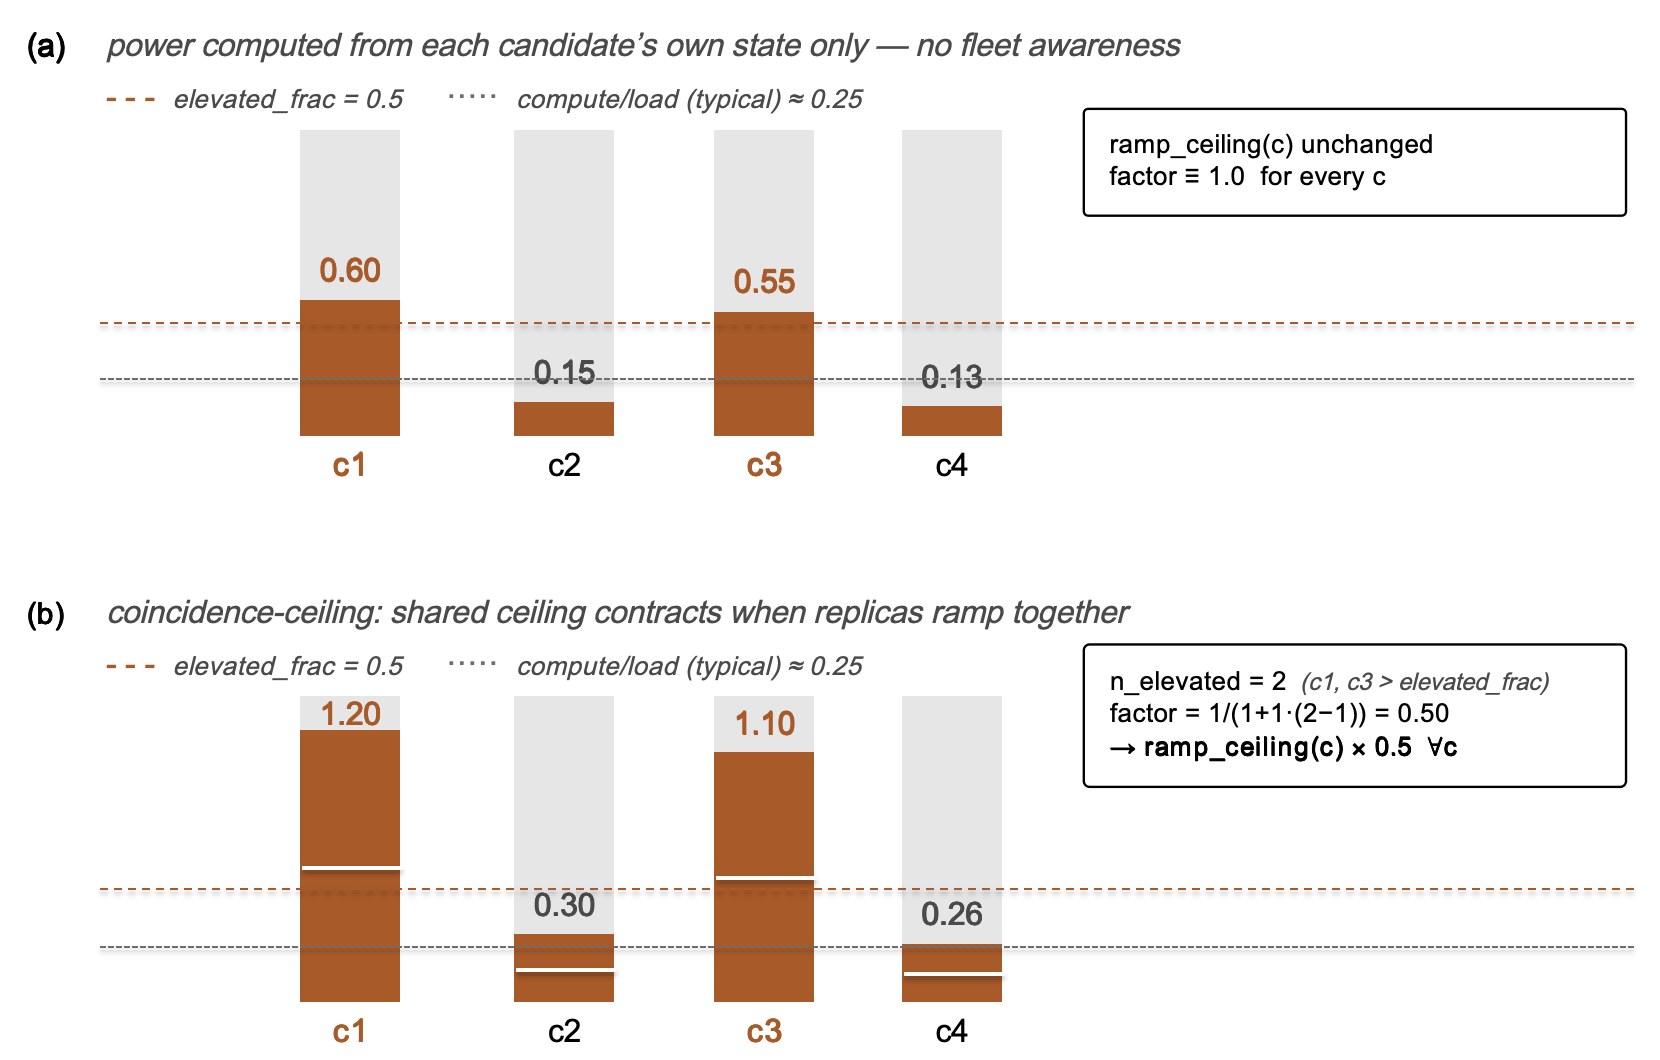
\includegraphics[width=0.9\linewidth]{figs/coincidence_ceiling.png}
  \caption{Four candidates' $\mathit{Share_{power}}$ (a) without and (b) with the
    coincidence-ceiling adjustment. Two candidates ($c_1$, $c_3$) exceed
    $\mathit{elevated\_frac}$, so $n_{\mathrm{elevated}}{=}2$ and the shared factor contracts
    every candidate's effective ceiling to $0.5\times$ --- doubling every candidate's
    $\mathit{Share_{power}}$ (white lines mark the unadjusted (a) values for comparison), not
    just the two that triggered it.}
  \label{fig:coincidence-ceiling}
\end{figure}

\textbf{No new proof needed.} The factor is one scalar, computed once per decision and shared
identically by every candidate at that decision --- exactly the object
Corollary~\ref{cor:ceiling-invariance} already covers, regardless of how the scalar is
computed. So $\mathit{drf\_power\_tiebreak\_full\_coincidence\_ceiling}$ inherits
Pareto-non-domination and threshold-safety from Corollary~\ref{cor:tiebreak-full-safe}/
Theorem~\ref{thm:threshold-safety} unchanged; $\mathit{weighted\_sum\_coincidence\_ceiling}$
inherits $\mathit{weighted\_sum}$'s Pareto-safety but not threshold-safety
(Theorem~\ref{thm:impossibility} still applies regardless of ceiling design);
$\mathit{lmetric\_power\_coincidence\_ceiling}$ inherits $\mathit{lmetric\_power}$'s lack of
Pareto-safety (Claim~\ref{claim:lmetric-power}'s cache-hit-collapse is orthogonal to which
ceiling feeds its power term). \textbf{The mechanism generalizes safety status; it does not
grant it.}

\textbf{This is not a no-op.} Scaling every candidate's ceiling by the same factor does not
change their relative order by $\mathit{Share_{power}}$ alone --- it changes
$\mathit{Share_{power}}$'s \emph{magnitude} relative to
$\mathit{Share_{compute}}$/$\mathit{Share_{load}}$ in $D(c) = \max(\ldots)$, making power more
likely to be the binding dimension for everyone during a genuine coincidence event. Verified
with a hand-constructed case that the mechanism actually flips a routing decision: without
adjustment, a replica with moderate local power pressure wins over one with zero power but
higher compute; with two \emph{other} replicas coincidentally elevated, the pick flips to the
higher-compute replica, avoiding piling onto an already-pressured fleet.

\textbf{Adopted rule.} We adopt $\mathit{drf\_power\_tiebreak\_full\_coincidence\_ceiling}$
(short-named $\mathit{coincidence\_ceiling}$) as this paper's proposed routing strategy: it is
the only coincidence-ceiling variant with a full, proven worst-case guarantee, inherited
without a new proof, and --- as \S\ref{sec:eval} shows --- empirically strong on the condition
central to this paper's motivation. We validate it against
$\mathit{lmetric\_power\_coincidence\_ceiling}$, the strongest empirically-performing
alternative found anywhere in this project's testing (Table~\ref{tab:rules}), rather than a
weaker unsafe foil.

\vspace{-3pt}
\section{Evaluation Methodology}
\label{sec:methodology}

\textbf{Setup.} 8$\times$4090 server (single chassis), 7B model
(Qwen2.5-Coder-7B-Instruct). Two independent NVML polling loops must not be conflated: the
router's own live power reads (computing $\mathit{Share_{power}}$) poll every 500\,ms; the
ground-truth power trace this paper's ramp/peak numbers come from is logged by a separate
sidecar targeting 50\,ms, actually ${\sim}89$\,ms once per-GPU NVML query overhead (six
replicas, queried in sequence) is accounted for --- a cheap live signal vs.\ a
higher-resolution offline trace, not interchangeable cadences.

Two further differences separate the decision-time signal from the numbers reported below,
neither a formal corollary of \S\ref{sec:formulation}--\S\ref{sec:coincidence-ceiling}'s
guarantees: (i) $\mathit{Share_{power}}$ clamps ramp rate non-negative (only a rising ramp is
routing-relevant), while the ramp statistics below use $|\Delta P / \Delta t|$, bidirectional;
(ii) $\mathit{Share_{power}}$ is per-replica, while ``peak power'' and ``mean/p99 ramp'' below
are fleet-aggregate (summed across all six GPUs), the physically meaningful grid-facing
quantity. Theorem~\ref{thm:threshold-safety} guarantees no avoidable violation of the
per-replica, upward-only quantity at decision time; the fleet-aggregate numbers are empirical,
not formally guaranteed.

$\mathit{Share_{power}}$'s ceiling $\kappa$ is calibrated \emph{per replica}: a dedicated check
(24 concurrent prefill bursts, isolated per GPU) found it varies \textbf{34\% across the six
replicas} (359.5--512.9~W/s) --- heterogeneity a shared constant would average away. Every
number here uses the corrected per-GPU ceiling; the old shared ceiling flipped or erased
apparent dominance in 4 of 6 tested conditions, always favoring an unsafe arm.

\subsection{The decision-level noise floor}
\label{sec:noisefloor}

Real hardware completion timing is not bit-reproducible across separate physical executions
(GPU kernel scheduling, thermal/clock variance, OS scheduling), so any state-dependent
router's live-state inputs ($\mathit{in\_flight\_after}$, $\mathit{ramp\_rate\_w\_per\_s}$)
are only ever ``true at this exact wall-clock instant,'' and that instant itself isn't
reproducible. Close-call ties get flipped by real timing noise a scoring formula cannot see,
and once one decision flips, replica loads genuinely diverge --- every subsequent decision
inherits a real, compounding state difference.

We quantified this directly by pairing individual routing decisions across independent runs
of the \emph{identical} policy on paired (fixed-seed) workload content, joined by conversation
id and turn (not row order, which real timing reshuffles for multi-turn conditions --- an
earlier, invalid attempt using naive row-order pairing gave misleadingly low mismatch numbers
on multi-turn conditions before this was caught and fixed). \textbf{Any state-dependent
routing rule mismatches on 75--85\% of individual decisions between two runs of itself}, with
the first divergence typically within the first ${\sim}35$ requests (median first-mismatch
row: 7). This holds across every condition tested, including two built entirely on real
conversation text with zero synthetic whale-padding (Light/Cachehit: 84.0--84.6\%; WildChat,
open-loop Poisson arrivals: 81.9--83.4\%) and a real-arrival-trace condition (BurstGPT:
75.0\%) --- ruling out synthetic workload construction, closed-loop feedback specifically
(WildChat is open-loop), and multi-turn interleaving artifacts as the cause.

\textbf{A state-blind control isolates the mechanism precisely.} $\mathit{round\_robin}$,
which never reads live replica state (only an incrementing counter), shows only
\textbf{3.1\% decision-mismatch} on the same condition where every load/power-aware rule
shows 75--85\%. This confirms the cause is state-dependence itself, not the evaluation
harness: any rule that reads live per-replica state is exposed to genuine, unavoidable timing
noise on real hardware; a rule that doesn't is nearly immune.

This is not a threat to dominance-based comparisons elsewhere in this paper --- dominance
requires simultaneous agreement across multiple metrics, which noise alone is unlikely to
produce consistently --- but it means any single-metric point estimate on a noise-sensitive
statistic (\S\ref{sec:metricselection}) between two low-trial-count arms should not be
over-read without checking it against a rule's own self-noise range first.

\subsection{Metric-selection principle: which statistics are trustworthy at feasible trial counts}
\label{sec:metricselection}

Not every aggregate statistic is equally exposed to the noise floor above. Metrics that
\textbf{sum or count over many independent events within a trial} are low-noise even at
$n{=}3$, while metrics that are \textbf{derivatives, extreme-value statistics, or spread over
few groups} are not --- a distinction that held consistently across every candidate metric
tested:

\begin{itemize}
  \item \textbf{Low-noise (survive $n{=}3$--6):} energy-per-token (total NVML-measured energy
    delta divided by total output tokens --- sums over on the order of $10^5$ tokens per
    trial) shows well under 1--3\% relative std across every arm and condition tested.
    SLO-violation-rate (fraction of requests exceeding fixed TTFT/TBT thresholds --- counts
    over hundreds of requests per trial) shows ${\sim}1.4$--2.3\%. Peak power, mean TTFT, and
    mean TBT --- themselves aggregate-ish quantities, not single-request point reads ---
    typically stay in the ${\sim}1$--2\% range at $n{=}3$, though noise level is
    condition-dependent rather than a fixed property of a given metric: TTFT's relative std is
    $0.4\%$ on the long condition but $6.2\%$ on the short condition this paper's headline
    comparison uses (\S\ref{sec:eval-dominance}), a $15\times$ difference. A plausible driver
    is that the short condition's shorter active window yields fewer within-trial TTFT samples
    to average cross-trial timing noise over, though this specific mechanism has not been
    independently verified.
  \item \textbf{High-noise (require 6+ trials, or should not be trusted for ranking claims at
    all at $n{=}3$):} mean/p99/max ramp rate --- derivatives or extreme-value statistics,
    sensitive to exact sample timing or a single worst event --- show 8--34\% relative std
    depending on which statistic. Two further candidates hypothesized to be
    integrated/fractional and therefore low-noise were tested and both failed:
    \textbf{coincidence-factor}
    (fraction of power-pressured time with 2+ replicas simultaneously elevated --- directly
    the quantity \S\ref{sec:coincidence-ceiling}'s mechanism targets) showed \textbf{56.97\%}
    relative std, worse than max\_ramp, because despite being a ``fraction'' it counts rare
    discrete threshold-crossing events (only hundreds of occurrences per trial), not the tens
    of thousands of samples that make energy-per-token stable. \textbf{Per-replica fairness
    CV} (dispersion of load/energy across only 6 GPUs) showed \textbf{32--40\%}, a
    small-$N$-groups problem structurally similar to estimating standard deviation from 3
    trials. ``Integrated'' or ``fractional'' alone does not guarantee low noise; what matters
    is the number of underlying events being summed.
\end{itemize}

A direct demonstration of why $n{=}3$ is insufficient for the high-noise tier: one arm's own
3-trial sample std on mean ramp was $\pm 1.7$~W/s; extending the same arm to 6 trials (same
condition) revealed a true std of $\pm 12.3$~W/s --- \textbf{$7\times$ larger}. Point estimates
and even sample standard deviations from 3 trials materially underestimate the true spread
for this class of metric.

\subsection{Trial-count implications, and closing the ``but the unsafe rule wins'' objection}
\label{sec:trialcount}

Applying \S\ref{sec:metricselection}'s principle retroactively to this project's own
empirical sweep: a full audit of the point-estimate range across 11 different routing rules
tested on the same condition found mean\_ramp's range spans only 2.12 true standard
deviations, p99\_ramp's 1.95$\sigma$, and max\_ramp's 1.17$\sigma$ --- \textbf{ranges this
narrow, across 11 independent samples, are exactly what pure sampling noise produces on its
own, no real difference between rules required to explain them.} This means most single-trial
or 3-trial ramp-statistic ranking claims from earlier in this project's investigation are not
currently statistically distinguishable from noise, and we do not assert them as confirmed
findings in \S\ref{sec:eval}.

We closed the most direct version of this objection --- ``the strongest unsafe alternative
performs better on ramp statistics, so the safety guarantee has a real cost'' --- by
replicating both $\mathit{coincidence\_ceiling}$ and
$\mathit{lmetric\_power\_coincidence\_ceiling}$ to matched $n{=}6$ on the same condition and
recomputing $z$-scores. \textbf{The apparent $n{=}3$ ramp-statistic edge for the unsafe rule
fully washed out at matched trial counts} ($z = -0.03$ to $+0.28$ on mean\_ramp, p99\_ramp,
and max\_ramp --- all statistically indistinguishable from zero), while energy-per-token was
already tied between them at $n{=}3$. \S\ref{sec:eval-matched} reports this comparison in
full.

This does not touch the theory: \S\ref{sec:formulation}--\S\ref{sec:coincidence-ceiling}'s
proofs are unaffected by any of this. It does mean this paper restricts its headline empirical
claims to the metrics independently confirmed low-noise in \S\ref{sec:metricselection} (peak,
TTFT, TBT, energy-per-token, SLO-violation-rate), applied uniformly regardless of which arm a
given metric happens to favor, rather than selectively including or excluding a statistic by
outcome, and to differences that clear a conventional significance threshold rather than
differences in point estimates alone (\S\ref{sec:eval-dominance}).

\vspace{-3pt}
\section{Experimental Results}
\label{sec:eval}

Main comparison restricted to four arms, per \S\ref{sec:coincidence-ceiling}/Table~\ref{tab:rules}'s
roles: $\mathit{coincidence\_ceiling}$ (proposed), $\mathit{lmetric}$ (power-blind baseline,
motivates why power-awareness matters at all), $\mathit{round\_robin}$ (state-blind baseline,
motivates why load-awareness matters), and $\mathit{lmetric\_power\_coincidence\_ceiling}$
(the strongest empirically-performing unsafe alternative, needed for the head-to-head that
closes the ``unsafe rule wins'' objection). Seven other arms tested this project (the
epsilon-shift Pareto-safe family, $\mathit{weighted\_sum\_coincidence\_ceiling}$,
$\mathit{compute\_only}$/$\mathit{load\_only}$, $\mathit{drf\_fixed}$) are discussed in
\S\ref{sec:counterexample}--\S\ref{sec:coincidence-ceiling} or noted in passing; full tables
are provided as supplementary material.

\subsection{Peak-power reduction on the short/original condition ($n{=}6$)}
\label{sec:eval-dominance}

Condition: closed-loop whale-injection traffic (15\% long-prompt fraction, 13.6--15.5k-token
whales), the paper's original validation condition. All four arms are replicated to
\textbf{$n{=}6$} (up from the $n{=}3$ used in earlier drafts of this project, per
\S\ref{sec:trialcount}'s recommendation), restricted to the three metrics
\S\ref{sec:metricselection} confirms are generally low-noise:

\begin{table}[t]
  \caption{Heavy/Closed-Loop (short), per-GPU-calibrated ceiling, mean $\pm$ std, $n{=}6$ for
    all four arms. Bold marks the lowest point estimate per row; significance is assessed
    separately in the text, not by this formatting.}
  \label{tab:headline}
  \footnotesize
  \setlength{\tabcolsep}{3pt}
  \begin{tabular}{@{}lrrrr@{}}
    \toprule
    Metric & \texttt{coincidence\_ceiling} & \texttt{lmetric} & \texttt{round\_robin} & \texttt{lp\_coincidence\_ceiling} \\
    \midrule
    Peak power (W)   & $\mathbf{2275.2{\pm}57.1}$ & $2388.2{\pm}31.9$ & $2321.6{\pm}53.8$ & $2318.2{\pm}74.8$ \\
    TTFT mean (s)    & $0.542{\pm}0.033$ & $0.560{\pm}0.032$ & $0.580{\pm}0.038$ & $0.537{\pm}0.038$ \\
    TBT mean (ms)    & $531.3{\pm}38.9$  & $544.2{\pm}48.9$ & $\mathbf{502.7{\pm}28.5}$ & $553.1{\pm}18.8$ \\
    \bottomrule
  \end{tabular}
\end{table}

Paired and unpaired $t$-tests ($n{=}6$, same fixed-seed workload content across trials)
confirm one of these three differences reaches conventional significance:
$\mathit{coincidence\_ceiling}$ reduces peak power by $4.7\%$ relative to $\mathit{lmetric}$
(unpaired $p{=}0.0017$, paired $p{=}0.0025$). The TTFT reduction relative to $\mathit{lmetric}$
is directionally consistent with the proposed rule but does not reach significance at $n{=}6$
(unpaired $p{=}0.36$, paired $p{=}0.10$), nor does the TBT reduction relative to
$\mathit{lmetric\_power\_coincidence\_ceiling}$ (unpaired $p{=}0.25$, paired $p{=}0.29$). The
confirmed result on this condition is the peak-power reduction; TTFT and TBT differences are
reported as directional, not as part of a multi-metric dominance claim.

\textbf{Against $\mathit{round\_robin}$, $\mathit{coincidence\_ceiling}$ is Pareto-incomparable
rather than dominant}: it wins peak power and, directionally, TTFT, but loses TBT ($531.3$
vs.\ $502.7$~ms). This pattern recurs throughout this project wherever $\mathit{round\_robin}$
is compared: a state-blind rule never concentrates load onto an already-busy replica, so it
cannot lose on tail-batching metrics like TBT the way a state-aware rule occasionally can,
even as it forgoes the gains available from reading load and cache state.

\textbf{Against $\mathit{lmetric\_power\_coincidence\_ceiling}$} --- the strongest
empirically-performing but Pareto-unsafe alternative, replicated here to matched $n{=}6$
(previously $n{=}3$) --- none of the three differences in Table~\ref{tab:headline} reach
significance (peak: unpaired $p{=}0.29$; TTFT: $p{=}0.80$; TBT: $p{=}0.25$). Combined with the
matched-$n{=}6$ ramp-statistic recheck (\S\ref{sec:eval-matched}) and the
energy-per-token/SLO-violation-rate comparison (\S\ref{sec:eval-efficiency}),
$\mathit{coincidence\_ceiling}$ is statistically indistinguishable from the strongest unsafe
alternative on every metric measured in this study --- direct evidence that the Pareto
guarantee is free, not merely that it avoids an efficiency cost. mean\_ramp/p99\_ramp/max\_ramp
are provided as supplementary material for completeness but are \textbf{not} part of this
confirmed claim, per \S\ref{sec:trialcount}'s uniform, outcome-independent restriction to
confirmed-low-noise metrics.

\begin{figure}[t]
  \centering
  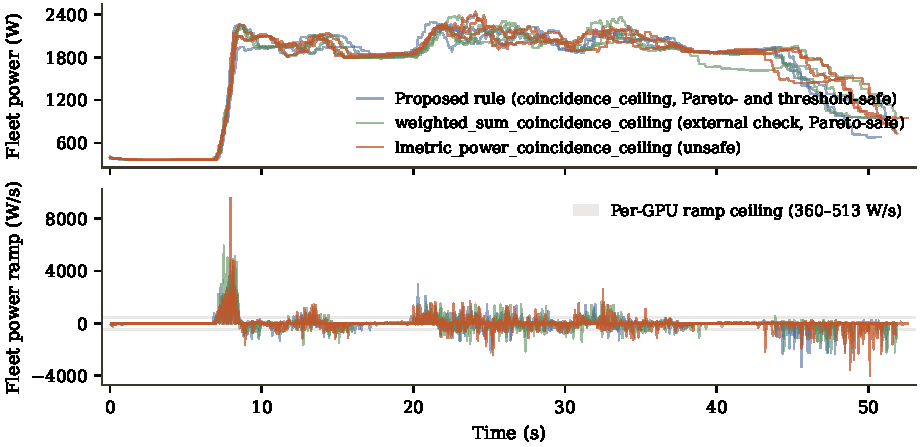
\includegraphics[width=\linewidth]{figs/ramp_comparison.pdf}
  \caption{Fleet-aggregate power (top) and its ramp rate (bottom), Heavy/Closed-Loop
    (short), 3 trials each of \texttt{coincidence\_ceiling} (proposed, Pareto- and
    threshold-safe), \texttt{weighted\_sum\_coincidence\_ceiling} (external validity check,
    Pareto-safe only), and \texttt{lmetric\_power\_coincidence\_ceiling} (unsafe), under the
    per-GPU-calibrated ramp ceiling (shaded band). The early ramp-up spike ($t{\approx}7$--$9$s)
    is where the three arms separate most: \texttt{lmetric\_power\_coincidence\_ceiling}'s
    worst per-trial peak ramp reaches $9575.0$~W/s, vs.\ $5955.8$~W/s for
    \texttt{weighted\_sum\_coincidence\_ceiling} and $4323.2$~W/s for the proposed rule ---
    a per-trial-max statistic that characterizes the trace, not a substitute for
    Table~\ref{tab:headline}'s significance-tested metrics. Away from that transient the three
    traces are visually close.}
  \label{fig:ramp-comparison}
\end{figure}

\subsection{Energy-per-token and SLO-violation-rate: the safety guarantee costs nothing}
\label{sec:eval-efficiency}

$\mathit{coincidence\_ceiling}$ does not reduce energy consumption --- a routing policy that
is work-conserving over the same request stream is not expected to change total energy
substantially, and this is not the claim made here. The claim is narrower: \textbf{the
Pareto-safety guarantee does not cost anything in efficiency or SLO compliance relative to the
strongest known unsafe alternative.}

\textbf{Energy-per-token} (total NVML $\mathit{energy\_mj}$ delta divided by total output
tokens, confirmed low-noise in \S\ref{sec:metricselection}): $\mathit{coincidence\_ceiling}$
beats $\mathit{round\_robin}$ on 6 of 7 conditions tested (often by 5--10\%). The one
exception, BurstGPT (7.7\% worse), is a known real-trace anomaly consistent with
earlier-documented project history (a real-BurstGPT-trace $\mathit{round\_robin}$ advantage
unrelated to whale-aware admission logic), not a new unexplained problem. Against
$\mathit{lmetric}$, results are mixed (clear wins on 4 conditions, ties or small losses
on 3). Against $\mathit{lmetric\_power\_coincidence\_ceiling}$ --- the comparison that matters
most for the ``guarantee costs nothing'' claim --- the two are statistically
indistinguishable on most conditions (e.g.\ $1.3132$ vs.\ $1.3051$ on the flagship long
condition, well within each other's noise).

\textbf{SLO-violation-rate} (fraction of requests with TTFT $>1.0$s or max TBT $>200$ms,
confirmed low-noise in \S\ref{sec:metricselection} --- though the fixed thresholds are
near-degenerate on lighter conditions where nearly every arm scores near 0\%, a real
limitation noted here and in \S\ref{sec:discussion}). TTFT-violation favors
$\mathit{coincidence\_ceiling}$ over $\mathit{round\_robin}$ on 5/7 conditions and over
$\mathit{lmetric}$ on 4/7. \textbf{TBT-violation is genuinely mixed}:
$\mathit{coincidence\_ceiling}$ loses to $\mathit{round\_robin}$ on Heavy/CL short ($0.2978$
vs.\ $0.2856$) and BurstGPT ($0.1627$ vs.\ $0.1683$), though it wins on WildChat ($0.5074$
vs.\ $0.5828$); it loses to $\mathit{lmetric}$ on Heavy/CL long ($0.3867$ vs.\ $0.3861$,
marginal) and WildChat ($0.5074$ vs.\ $0.4134$, a real loss). The tail-latency result of this
paper is a peak-power win on the flagship condition (\S\ref{sec:eval-dominance}) and a
directionally favorable TTFT picture more broadly, not a universal win on every latency
statistic.

\begin{table}[t]
  \caption{Energy-per-token, headline arms, all 7 conditions (mean $\pm$ std, J/token).
    SLO-violation-rate figures for all 7 conditions and 4 arms are provided as supplementary
    material; the figures behind the disclosure above are cited inline.}
  \label{tab:energyslo}
  \footnotesize
  \setlength{\tabcolsep}{3pt}
  \begin{tabular}{@{}lrrrr@{}}
    \toprule
    Condition & \texttt{coincidence\_ceiling} & \texttt{lmetric} & \texttt{round\_robin} & \texttt{lp\_coincidence\_ceiling} \\
    \midrule
    Heavy/CL short  & $1.4242{\pm}0.0193$ & $1.4180{\pm}0.0222$ & $1.4395{\pm}0.0176$ & $1.4179{\pm}0.0230$ \\
    Heavy/CL long   & $1.3132{\pm}0.0050$ & $1.3251{\pm}0.0242$ & $1.3363{\pm}0.0023$ & $1.3051{\pm}0.0032$ \\
    Heavy/Matched   & $0.7393{\pm}0.0116$ & $0.7510{\pm}0.0110$ & $0.7486{\pm}0.0075$ & $0.7456{\pm}0.0040$ \\
    Light/Cachehit  & $1.2287{\pm}0.0028$ & $1.2517{\pm}0.0102$ & $1.2944{\pm}0.0042$ & $1.2339{\pm}0.0021$ \\
    BurstGPT        & $2.8070{\pm}0.0312$ & $2.8599{\pm}0.0235$ & $2.6059{\pm}0.0118$ & $2.8403{\pm}0.0101$ \\
    Ramp \& Route   & $2.2950{\pm}0.0323$ & $2.2537{\pm}0.0187$ & $2.5404{\pm}0.0462$ & $2.2508{\pm}0.0373$ \\
    WildChat        & $0.3227{\pm}0.0071$ & $0.3147{\pm}0.0045$ & $0.3448{\pm}0.0004$ & $0.3146{\pm}0.0060$ \\
    \bottomrule
  \end{tabular}
\end{table}

\subsection{Matched $n{=}6$ recheck against the strongest unsafe alternative}
\label{sec:eval-matched}

Per \S\ref{sec:trialcount}, both $\mathit{coincidence\_ceiling}$ and
$\mathit{lmetric\_power\_coincidence\_ceiling}$ were replicated to matched $n{=}6$ on the
flagship condition, and $z$-scores were recomputed on the three ramp-derivative statistics:
$z = -0.03$ to $+0.28$ on mean\_ramp, p99\_ramp, and max\_ramp, all statistically
indistinguishable from zero. The apparent $n{=}3$ advantage for the unsafe rule does not
survive matched replication. This result extends to peak power, TTFT, and TBT as well
(\S\ref{sec:eval-dominance}) and to energy-per-token and SLO-violation-rate
(\S\ref{sec:eval-efficiency}): on every metric this study measures, at matched trial counts,
giving up the Pareto guarantee produces no statistically distinguishable empirical advantage.

\subsection{Alternative Share\_power Definitions}
\label{sec:eval-sharepower}

Two alternative $\mathit{Share_{power}}$ definitions were evaluated against the deployed raw
two-point derivative: an EMA-smoothed estimate ($\alpha{=}0.3$), and a retarget to
instantaneous peak power. Smoothing reduces the signal's own relative std by 18--53\% but not
a consistent downstream improvement: it beats $\mathit{coincidence\_ceiling}$ on
energy-per-token on 3 of 7 conditions and loses on 4; max\_ramp is worse on 6 of 7, and Ramp \&
Route loses across five metrics at once. The peak-power retarget regresses sharply on the two
conditions tested so far (energy-per-token $+11\%$, TTFT-violation nearly $2\times$,
TBT-violation $+21\%$), and changes the mechanism's physical target from grid-transient
avoidance to capacity/thermal management, a different problem. Neither alternative is adopted;
raw ramp-rate is retained on both empirical and mechanistic grounds.

\vspace{-3pt}
\section{Discussion and Limitations}
\label{sec:discussion}

\begin{itemize}
  \item \textbf{Small-$N$ / shared-PDU caveat}: 8$\times$4090 in one chassis likely shares
    upstream PDU/PSU, not independent grid circuits. A data-center-scale claim needs a separate
    extrapolation model, deliberately not attempted: a sibling project retracted its own
    fleet-scale extrapolation after a parametric Monte Carlo model (P99 ramp tail
    underestimated ${\sim}5.8\times$ against hardware) and a model-free trace-bootstrap
    (tail-statistic sign flips from a small segment library) both failed on tail fidelity, with
    a \emph{thicker} trial library than this project's (3--6 trials/arm).
  \item \textbf{Real-signal losses, disclosed rather than omitted}: on the long/sustained-pressure
    condition, $\mathit{coincidence\_ceiling}$'s mean\_ramp is significantly higher than
    $\mathit{round\_robin}$'s ($z{\approx}{+}2.82$, $n{=}6$), credible given mean\_ramp is the
    \emph{least} noisy ramp derivative (\S\ref{sec:metricselection}).
    \S\ref{sec:eval-efficiency}'s TBT-violation-rate picture is mixed against both baselines.
    BurstGPT's energy-per-token reverses ($\mathit{coincidence\_ceiling}$ 7.7\% worse than
    $\mathit{round\_robin}$), consistent with an earlier-documented, still-undiagnosed
    real-BurstGPT anomaly.
  \item \textbf{Scope of validation}: the confirmed peak-power result (\S\ref{sec:eval-dominance})
    is on the short/original condition; the long/sustained-pressure condition shows no
    confirmed ramp-safety advantage in either direction, and the tail-latency result is not
    claimed to generalize beyond conditions where confirmed, while the efficiency/SLO
    no-regression result holds broadly (\S\ref{sec:eval-efficiency}). Which workload
    properties predict where the peak-power win holds is future work.
    $\mathit{Share_{power}}$'s live-signal ablations (\S\ref{sec:eval-sharepower}) are partial:
    the peak-power retarget has data on 2 of 7 conditions so far.
  \item \textbf{Per-decision vs.\ per-trajectory, per-replica vs.\ aggregate}:
    \S\ref{sec:formulation}'s welfare objective is myopic; a sequence of decisions is not
    claimed optimal over a trajectory, only that each satisfies a static guarantee.
    Fleet-aggregate ramp sums across replicas, so a per-replica bound does not mechanically
    bound the sum --- \S\ref{sec:coincidence-ceiling}'s mechanism targets the aggregate hazard
    directly, still inheriting the per-decision proof, but no formal bound on the aggregate
    trajectory is claimed, only the empirical characterization in \S\ref{sec:eval}.
  \item \textbf{Fixed replica pool}: this paper routes among $N$ already-running replicas;
    which replicas are powered on is a separate, coarser-timescale problem not addressed here.
\end{itemize}

\vspace{-8pt}
\section{Related Work}
\label{sec:relatedwork}

\begin{itemize}
  \item \textbf{Dominant Resource Fairness (DRF)}~\cite{ghodsi2011drf} --- multi-resource fair
    allocation via lexicographic comparison of dominant shares, proven Pareto-efficient for
    static per-user demand vectors. We extend the resource set to a third, live/reactive
    dimension (\S\ref{sec:formulation}) and re-derive Pareto-efficiency for this dynamic
    setting.
  \item \textbf{LMETRIC}~\cite{zhang2026lmetric} --- multiplicative $\mathit{P\text{-}token}
    \times \mathit{BS}$ scoring for LLM-serving load balancing, a simpler non-fairness-theoretic
    baseline. \S\ref{sec:counterexample} shows a power-extended form sacrifices the Pareto
    guarantee via a distinct mechanism from the DRF-family variant; \S\ref{sec:eval}'s
    validation is a head-to-head against its coincidence-ceiling-extended form, the strongest
    empirical performer found here.
  \item \textbf{Power-aware ML system design (Zeus, Perseus)}~\cite{you2023zeus,
    chung2024perseus} --- tune per-job GPU frequency/power (Zeus) or schedule energy across
    pipeline stages (Perseus) \emph{within} a training job, via DVFS. $\mathit{ramp\_ceiling}$
    (\S\ref{sec:formulation}) is physically a DVFS symptom, treated here as measured
    (\S\ref{sec:methodology}) not controlled. This paper acts at a different layer --- which
    replica serves a request, not a GPU's own DVFS state --- and the two compose.
  \item \textbf{Power-of-Two-Choices}~\cite{mitzenmacher2001power,azar1994balanced} ---
    sampled load balancing with a proven exponential improvement in expected max load; a
    different mechanism family (randomized sampling vs.\ our deterministic rule).
  \item \textbf{Power capping as an alternative mechanism}~\cite{ma2026illusion} --- GPU-level
    caps are often \emph{inert} for decode-dominated LLM serving (137--300~W on a 700~W GPU)
    since a facility-level cap frequently never engages, motivating acting upstream instead.
  \item \textbf{Grid-integrated infrastructure \& switching costs}~\cite{chien2026sustainability,
    li2025fairness, astrom2008feedback} --- broader grid-aware AI workload strategies operate
    at a coarser, facility/life-cycle timescale than this paper's per-request (500\,ms) layer,
    which addresses intra-fleet spikes, not grid-scale coordination. $\mathit{Share_{power}}$'s
    ramp-rate term is conceptually a switching-cost signal and $\mathit{ramp\_ceiling}$ a
    slew-rate bound whose set-point \S\ref{sec:coincidence-ceiling} estimates online;
    \S\ref{sec:lemma1}'s guarantee is per-decision, unlike that literature's
    regret/competitive-ratio analysis.
\end{itemize}

\vspace{-8pt}
\section{Conclusion}

This paper gives power-aware LLM-serving routing a theoretical grounding and a single
proposal: $\mathit{drf\_power\_tiebreak\_full\_coincidence\_ceiling}$, a sorted-lexicographic
DRF rule extended with a pluggable coincidence-ceiling mechanism targeting the
fleet-\emph{aggregate} coincident-ramp hazard no per-replica rule can see, at no additional
proof cost. On real 8$\times$4090 hardware it delivers a significant peak-power reduction over
a power-blind baseline ($p{=}0.0017$, $n{=}6$) and matches the strongest unsafe alternative on
every metric measured at matched $n{=}6$ --- the guarantee costs nothing tested. A second
contribution: a ${\sim}75$--85\% decision-level noise floor inherent to real-hardware
closed-loop evaluation, and the methodology for judging which claims here can be trusted.

\bibliographystyle{ACM-Reference-Format}
\bibliography{references}

\end{document}
